\chapter{ Констукторский раздел}
\label{cha:design}
    В данном разделе будут рассмотрены схемы алгоритмов, требования к функциональности ПО, и определены способы тестирования.
    
    \section{Описание структур данных}
        В данной работе линии вычислительного конвейера реализованы с помощью очереди [\ref{bib:4}], реализованной на одномерном динамическом массиве. Выбор типа данных обусловлен тем, что заявки обрабатываются в порятке их поступления, выполнив их последовательно.
	
	\section{Схемы алгоритмов}
        Ниже будут представлены схемы алгоритмов: \begin{enumerate}
            \item работы конвейера (рисунок \ref{schema:Pipeline});
            \item XOR-шифра (рисунок \ref{schema:Xor});
            \item шифра Цезаря (рисунок \ref{schema:Caesar}).
        \end{enumerate}
      
       	    \begin{figure}[h!]
       		\centering
       		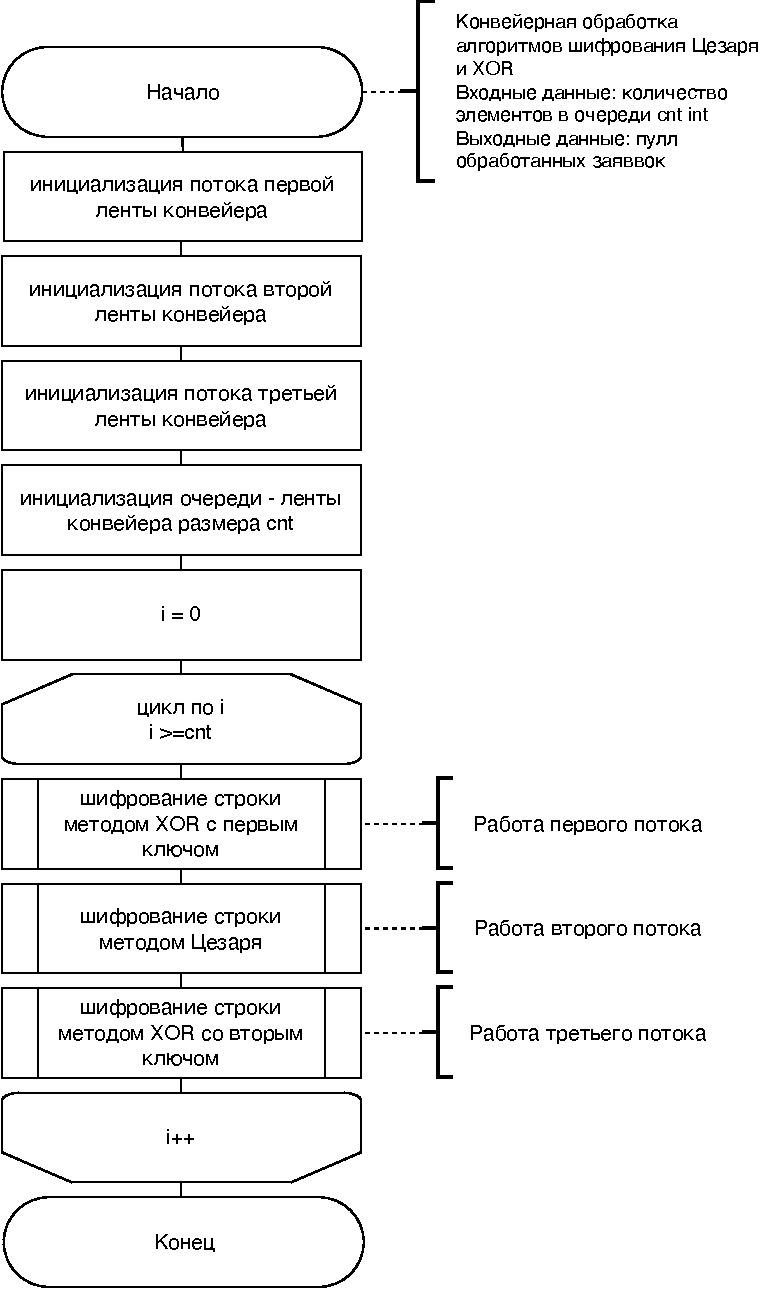
\includegraphics[scale=0.8]{Pipeline.pdf}
       		\caption{Схема работы конвейера}
       		\label{schema:Pipeline}
       	\end{figure}\clearpage
        \begin{figure}[h!]
            \centering
            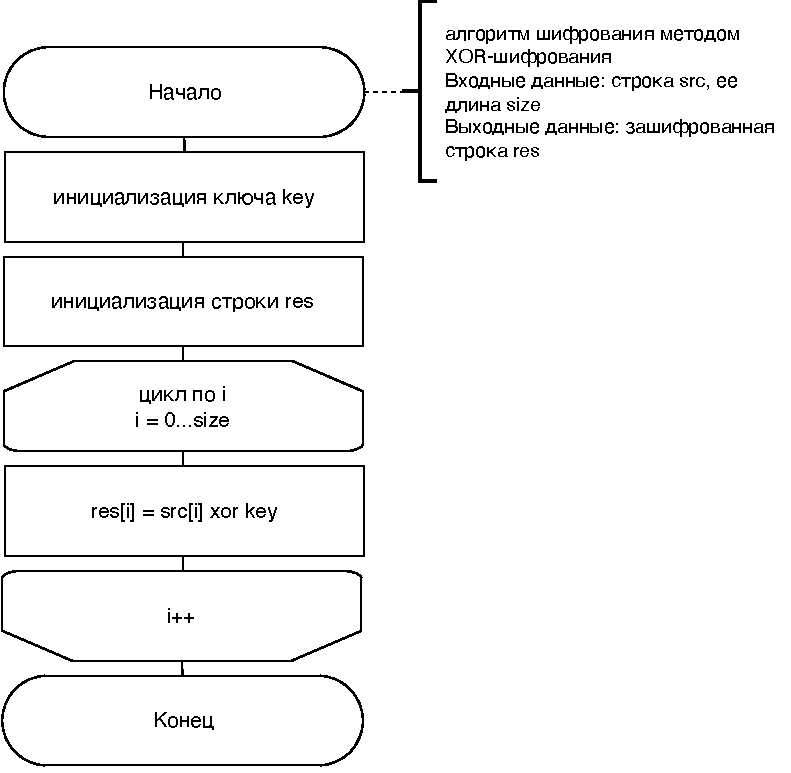
\includegraphics[scale=0.8]{Xor.pdf}
            \caption{Схема алгоритма XOR-шифра}
            \label{schema:Xor}
        \end{figure}\clearpage
        \begin{figure}[h!]
            \centering
            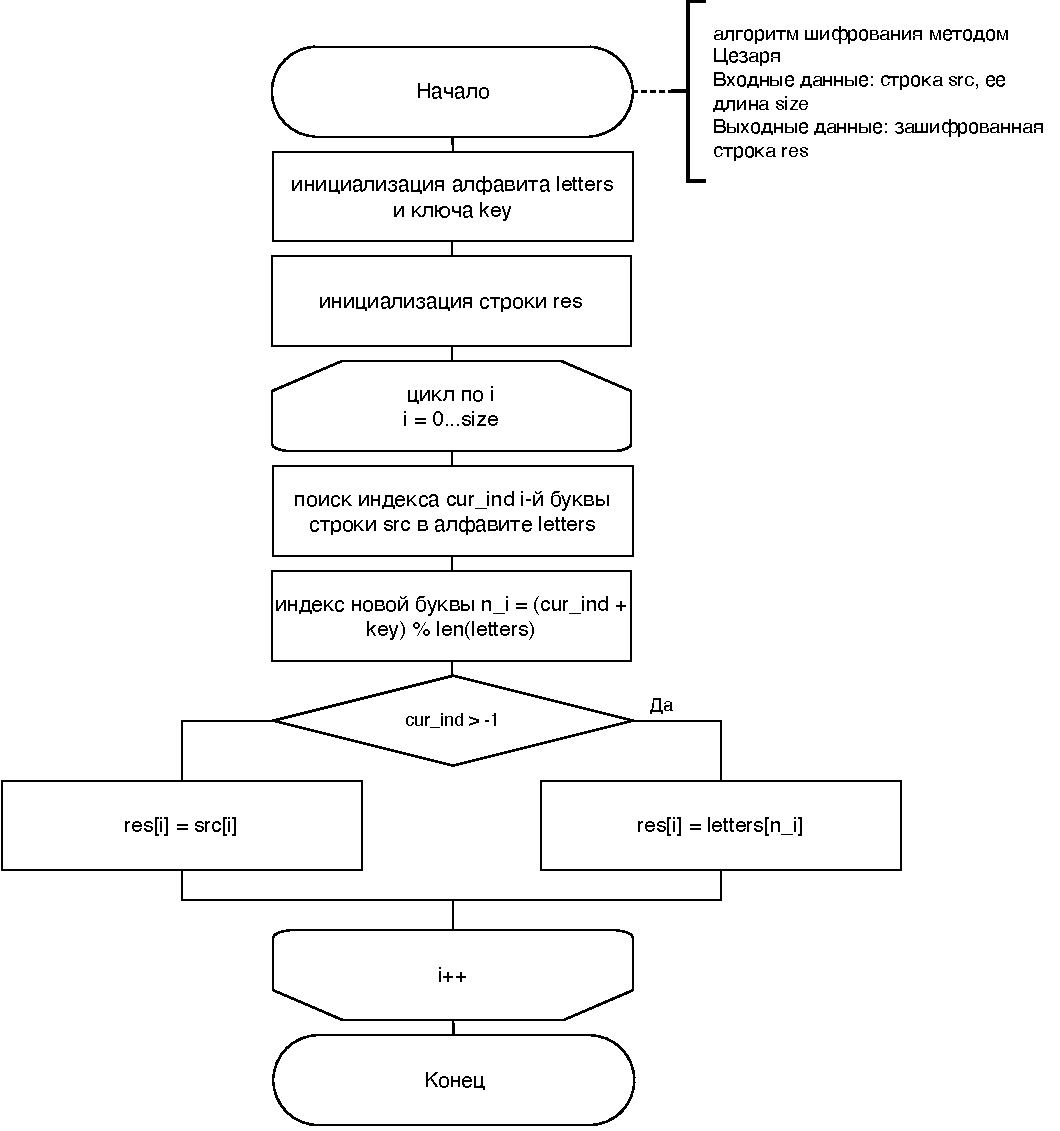
\includegraphics[scale=0.8]{Caesar.pdf}
            \caption{Схема алгоритма шифрования методом Цезаря}
            \label{schema:Caesar}
        \end{figure}\clearpage

        

    \section{Структура ПО}
    \par Программа поделена на ряд смысловых модулей, описанных ниже:
    \begin{itemize}
        \item Модуль «chiperalg», в котором содержатся процедуры и функции, связанные с алгоритмами шифрования и генерации строк;

        \item Модуль «pipeline», в котором содержатся функции работы параллельного и синхронного конвейера, функции работы с очередью и журналирование.
    \end{itemize}

    Программа имеет консольный интерфейс.

	\section*{Вывод}
    \par Были разработаны схемы алгоритмов, необходимых для решения задачи. Получено достаточно теоретической информации для написания программного обеспечения.
\newpage